\section{Hướng tiếp cận}

Đã có một số báo cáo tương tự chỉ ra vấn đề chung của phương pháp học trình tự với mạng nơ-ron. Cách tiếp cận trong bài báo này thì gần với \citep{kalchbrenner2013recurrent}, người đầu tiên nghiên cứu giải thuật ánh xạ toàn bộ câu đầu vào thành vectơ và tương tự như \citep{cho2014learning} mặc dù sau này chỉ được sử dụng để phục hồi các giả thuyết được tạo ra bởi một hệ thống dựa trên cụm từ. Graves \citep{graves2015generating} đã giới thiệu kỹ thuật attention cho phép mạng nơ-ron tập trung vào các phần khác nhau trong đầu vào của chúng và một biến thể của ý tưởng này đã được Bahdanau áp dụng thành công cho việc dịch máy \citep{bahdanau2019neural}. Phân loại trình tự kết nối là một kỹ thuật phổ biến khác để ánh xạ các trình tự thành các trình tự có mạng nơron, nhưng nó giả định một sự liên kết đơn phương giữa các đầu vào và đầu ra \citep{graves2006connectionist}.

\begin{figure}
	\centering
	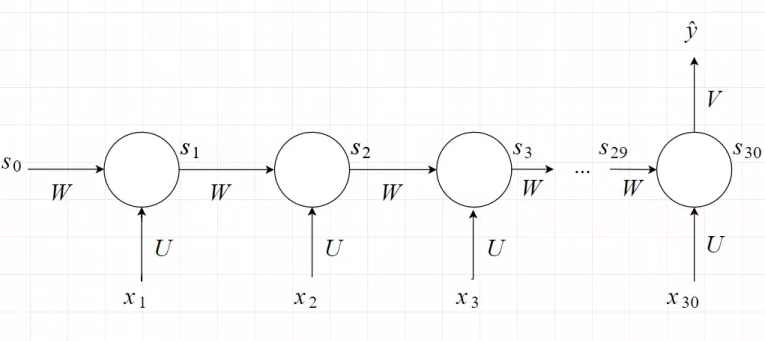
\includegraphics[scale=0.3]{img/rnn.png}
	\caption{Mô hình RNN}
	\label{rnn}
\end{figure}

Mô hình đề xuất dựa trên mô hình mạng nơ-ron sâu LSTM, đây là một dạng đặc biệt của RNN (Recurrent Neural Network - Mạng nơ-ron hồi quy). LSTM được giới thiệu bởi \citep{HochreiterandSchmidhuber1997} nhằm giải quyết các bài toán về phụ thuộc xa (long-term dependency). Ý tưởng là sử dụng một LSTM để đọc chuỗi đầu vào, một bước thời gian tại một thời điểm, để biểu diễn vectơ có chiều cố định lớn và sau đó sử dụng một LSTM khác để trích xuất chuỗi đầu ra từ vectơ đó. LSTM thứ hai về cơ bản là một mô hình ngôn ngữ mạng nơ-ron hồi quy \citep{Mikolov2010} ngoại trừ việc nó được điều chỉnh dựa trên chuỗi tuần tự đầu vào. Khả năng học thành công trên dữ liệu có phạm vi dài phụ thuộc vào thời gian của LSTM khiến nó trở thành lựa chọn đương nhiên cho ứng dụng này do độ trễ thời gian đáng kể giữa đầu vào và đầu ra tương ứng của chúng.

\begin{figure}
	\centering
	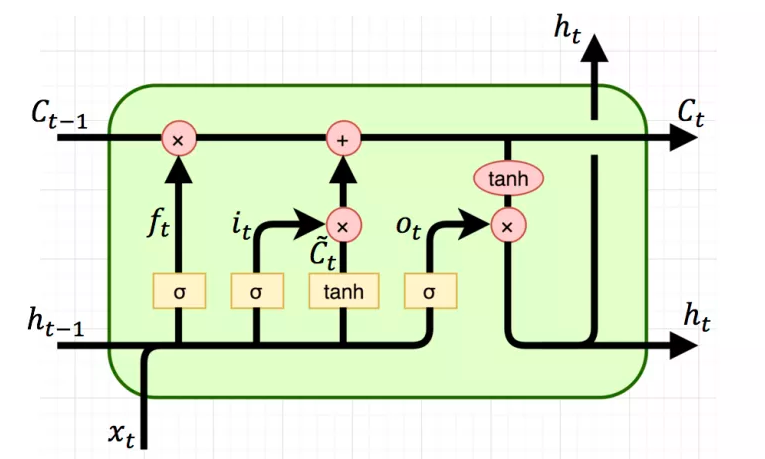
\includegraphics[scale=0.3]{img/lstm.png}
	\caption{Mô hình LSTM}
	\label{lstm}
\end{figure}